\documentclass{article}

\usepackage[utf8]{inputenc}

\usepackage{graphicx}
\usepackage{subcaption}
\usepackage{mathtools}
\usepackage{wrapfig}
\usepackage{graphicx}
\usepackage{subcaption}
\usepackage{mathtools}
\usepackage{wrapfig}
\usepackage{float}
\usepackage{gensymb}
\usepackage{caption}
\usepackage{geometry}
\usepackage{cite}

\DeclareMathOperator{\sech}{sech}
\DeclareMathOperator{\Tr}{Tr}

\usepackage{listings}
\usepackage{color}

\definecolor{codegreen}{rgb}{0,0.6,0}
\definecolor{codegray}{rgb}{0.5,0.5,0.5}
\definecolor{codepurple}{rgb}{0.58,0,0.82}
\definecolor{backcolour}{rgb}{0.95,0.95,0.92}
 
\lstdefinestyle{mystyle}{
    backgroundcolor=\color{backcolour},   
    commentstyle=\color{codegreen},
    keywordstyle=\color{magenta},
    numberstyle=\tiny\color{codegray},
    stringstyle=\color{codepurple},
    basicstyle=\footnotesize,
    breakatwhitespace=false,         
    breaklines=true,                 
    captionpos=b,                    
    keepspaces=true,                 
    numbers=left,                    
    numbersep=5pt,                  
    showspaces=false,                
    showstringspaces=false,
    showtabs=false,                  
    tabsize=2
}

%\usepackage{minted}
%\begin{minted}{haskell}
 
\lstset{style=mystyle}





\makeatletter
\renewcommand\paragraph{\@startsection{paragraph}{4}{\z@}%
	{-2.5ex\@plus -1ex \@minus -.25ex}%
	{1.25ex \@plus .25ex}%
	{\normalfont\normalsize\bfseries}}
\makeatother
\setcounter{secnumdepth}{4} % how many sectioning levels to assign numbers to
\setcounter{tocdepth}{4}    % how many sectioning levels to show in ToC in preamble





\geometry
{
  %body={6.5in, 8.5in},
  left=1.0in,
  top=1.25in
}

\setlength{\parindent}{10ex}









%\begin{figure}[H]
%	\centering
%	\includegraphics[scale=0.2]{rhul_logo}
%\end{figure}











%%%%%%%%%%%%%%%%%%%%%%%%%%%%%%
%Re-Write intro

%Re-Write Background, example emergence so it feels less like an aside. Give enough detail of Interdyne that it can be used later when creting the transfromation desgin 

%Add to the description and alays what the challanges are 

%Write RR langauge section 

%Write Convertor section 

%Write Validation

%Wrtie test 

%Write Conclusion and further work 


\begin{document} 
\title{Correctness-Preserving Translation from First Order Recurrence Relation to an Agent-Based Representation} 
\author{Leo Carlos-Sandberg\\
Supervisor: Dr Christopher D. Clack} 
\maketitle 

\begin{abstract}
\noindent {\it 
This paper investigates a method of describing interacting systems from two opposing view points, recurrence relations and agent-based models. These two methods take fundamentally different approaches with recurrence relations being top-down, and agent-based models being bottom-up.\\
Connecting these two methods allows for a more complete investigation of emergent behaviour occurring within interacting systems. Agent-based models offer an attractive way of analysing emergent behaviour, with the ability to investigate individual interactions as message passing throughout a simulation. Agent-based models however tend to be less well understood and accepted by those outside computer science, this is in contrast to recurrence relation which are normally well understood. Creating a correctness preserving link between recurrence relations and agent-based models allows for simulations to be understood in their recurrence relation representation and hence have their agent-based model representation accepted. This is important in fields such as finance as it opens up new tools for economists and regulators to use in understanding emergence in complex markets.\\
This research comprises the definition of a simple recurrence relation language, to define simulations, and the design of a step-by-step process by which a set of recurrence relations defined in this language can be converted into an agent-based model representation, the InterDyne simulator is chosen as a target representation for this transformation. 

}
\end{abstract}




\newpage
\newgeometry{top = 2cm}
\tableofcontents
{\textit{ }}
\restoregeometry
\newpage



%\begin{figure}[H]
%	\centering
%	\includegraphics[scale=0.5]{spin_on_lattice}
%	\caption{\it The two-dimensional Ising model lattice.}
%	\label{fig:spins_on_lattice_demo}
%\end{figure} 

%\begin{equation}
%E = -J\sum_{\langle i,j \rangle}^{N} s_{i}s_{j} - h \sum_{i = 1}^{N} s_{i}.
%\end{equation}

%\label{1d_code}

%~\cite{GouldBook} 
%~\ref{s_the_ising_model} 

%%%%%%%%%%%%%%%%%%%%%%%%%%%%%%%%%%%%%%%%%%%%%%%%%%%%%%%%%%%%%%%%%%%%%%%%%%%%%%%%%%%%%%%%%%%%%%%%%%%%%%%%%%%%%%%%%%
\section{Introduction}
Complex systems have been an area of deep interest for a long time in many  fields such as, physics, biology and chemistry. More recently this is true in the fields of economics and finance, especially as the markets have become increasingly automated and interconnected. These systems can exhibit unexpected and hard to predict behaviour, known as emergence, which can some times, have a large impact and damage a system.\\ 
Emergent behaviour can occur in a large number of ways, but more often the behaviour of interest is created over a time period. In general there are two ways of viewing systems in time, these are either continuous, where the system progress through time smoothly. Or discrete, where the system takes equal quantised steps through time, with each step advancing the system.\\
For discrete time systems two particular modelling techniques that can be used are, recurrence relations and agent-based models. These two methods take fundamentally different views of a system, recurrence relations take a top down view and can be seen as a set of mathematical equations which make calls for the values of each other. Agent-based models take a bottom up approach and model different elements of the system as individual agents which communicate via messages passed between each other.\\
Both of these techniques have been extensively used in the modelling of complex systems, in a larger range of fields [REFS???]. %REFS????
Recurrence relations have a number of advantages such as:
\begin{itemize}
%  \item Being well understood in a large number of fields. 
  \item Giving a formal mathematical definition of the whole system.
  \item Showing an obvious link between equations within the system. 
  \item Giving a static representation of the system.  
\end{itemize}
Agent-based modelling benefits include:
\begin{itemize}
  \item Being able to encode unique agents, with varying levels of complexity.
  \item Not having a defined behaviour for the system as a whole, as it is a bottom up approach.
  \item Giving a dynamic representation of the systems evolution. 
  \item Plainly showing the passing of information between agents. 
\end{itemize}          
The ability of agent-based models to track the communication between agents and their bottom up approach makes them particularly adapt at analysing emergent behaviour.\\  
As mentioned there has been a growing interest into complex systems and emergence in finance, a large part of this interest is on regulating theses systems to stop the creation of destructive emergent behaviour. This has been especially true when looking at high-frequency trading, which has been accused of causing a number of negative effects within the markets, including flash crashes. This trading takes place at high speeds comparable to the tickets on a computers internal clock, meaning models of this type of trading typically will take a discrete time approach.\\
Though both agent-based model and recurrence relations have been used within finance, there is a notable preference among researchers grounded in economics to use recurrence relations, shown in Section~\ref{litreviewofabmrr}. This preference appears to be caused by agent-based models not resonating with these researchers, leading to them passing over using the models as well as results be other researchers using the models being less widely accepted.\\
This lack of acceptance presents a problem for work on emergence within the financial system, agent-based models are a strong tool in investigating emergent behaviour, ignoring them seriously limit the ability to research this area, and a large amount of research has already been done in this area using agent-based model, if this work is only accepted by a subsection of the community its impact will be substantially lessened.\\     
This paper seeks to present a method where by agent-based models will resonate better with experts such as economists, and hence that they will be used more frequently and the research based upon them will be better accepted.\\    
This raises the question, how can agent-based models be explained to a sceptic in such a way that they will accept them? This papers approach is to connect agent-based models and recurrence relations together, allowing the already accepted recurrence relations to become the formalism of the agent-based model.\\ 
For this approach to work, there has to be confidence that the connection between the recurrence relations and agent-based model, has a significance and is correct. Hence the next question is what is a meaningful connect? A correctness preserving transformation was chosen as a connection, allowing the recurrence relations and agent-based model to be two views of the same system, hence giving meaning to the agent-based model of the system in terms of recurrence relations. This approach is coined as the two views \\    
This transformation takes a set of recurrence relations and turns them into an agent-based model, this direction has been chosen opposed to the reverse as the aim is to encourage sceptics to engage with agent-based models, so allows them to start with the familiar before the transformation.\\ 
To achieve this transformation from a set of recurrence relations to a agent-based model, a number of conceptual challenges needed to be addressed. These problems are discussed in greater depth in Section~\ref{twoviewsapproach} but including: 
\begin{itemize}
   \item The two paradigms of the models are completely different and opposing. 
   \item How are function calls related to message passing?
   \item How can the idea of agents having a infinite list through out time of their values be derived from the recurrence relations? 
   \item How can the idea of private and public information introduced, and what data should fall into each category? 
   \item How can public broadcast data be introduce, and what data classifies to be treated as such? 
   \item How can time limited information be introduced?
   \item How can name control be introduced in a tangible way into a recurrence relations that have no notion of agents. 
   \item How can output messages containing message information be introduced? 
   \item How can the recurrence relations be split in a way which does not splinter the model? 
   \item How can small, and hence more susceptible to prove of correctness, steps be used to transform the model? 
\end{itemize}
To create a transformation that allows these issues to be overcome and to increase the easy in proofing the correctness of this conversion, a step-by-step approach was taken, where the transformation is done in a series of small correctness preserving steps.\\  
This papers aim is hence to create the design of each of these steps, in the process of transforming from a set of recurrence relations to an agent-based model.\\ 
Creating this transformative method has  two important aspects, increasing the acceptance of agent-based models and creating a model for viewing systems in two perspectives. Increasing the acceptance of agent-based models has a number of benefits including: 
\begin{itemize}
   \item Increasing the use of agent-based models in new research, where their benefits would be more suited. Hence increasing the ease in which emergence can be investigated within the financial system. 
   \item Allow for work already done using agent-based models to be re-evaluated with a greater understanding to the methods used. 
\end{itemize}
The creation of the two views model always a number of unique benefits by providing a new tool for analyse of complex systems: 
 \begin{itemize}
    \item Adds a new technique for viewing and modelling complex systems.
    \item Adds a new tool that can be used for hypotheses formalisation and communication of ideas between researchers. 
    \item Adds a model that is suitable for both static and dynamic analyses. 
 \end{itemize}
The timing of this paper fits with the increased interest in agent-based models within finance, for modelling the complex behaviour of the markets [REFS???????]. %REFS????
This work is designed to be able to support other work done using agent-based models and help further the understanding of agent-based models during this time of interest.\\
To show a conversion between the two types of models a particular example of each must be chosen, for this paper a custom recurrence relation language was designed to be transformed into the agent-based model known as InterDyne. InterDyne was chosen in particular due to it being designed from the bottom up to model and investigate emergent behaviour within the financial markets, this software was also a convenient choice due to access to the source code and local expertise.\\    
This papers layout is as follows. First a background is given detailing, emergent behaviour generally and in the financial markets, a description and review of the literature of both recurrence relations and agent-based models, and a in-depth description of InterDyne. Secondly a description and analysis of the problems with agent-based models and how a two-view approach addresses them. Thirdly a description of the design, formal syntax, and use, of the custom recurrence relation language. Fourthly the design and a example of the step-by-step transformation between the two models. Fifthly a validation that the transformed example does indeed represent a InterDyne simulation. Sixthly a test of a number of examples for correctness of functionality. Lastly the paper is concluded and summarised with notes for further work given.     
%This connection between the models is coined as the two-views approach.\\



%regulation is shifting from micro to macro-prudential perspective 
%managing individual risk to managing systemic risk

%USE THIS LINK
%\cite{fallacyofcompostionBook}
%talks about policy due to emergence 
%page 10 
%googled "fallacy of division emergent behaviour"

%no formal description of the problem

%-DEVS model does give you overarching symatic (why is it not approate to model interarction dynamics) 



%Compare difference equations and ABM in intro using the "TO AGENT-BASED SIMULATION FROM SYSTEM DYNAMICS" paper



%in project scope: show some limited implementation. Say initial aim was to design, but not implement the translation steps. However, the project has succeeded in all of the design aims and additionally succeeded in implementing several of the translation steps."













%%%%%%%%%%%%%%%%%%%%%%%%%%%%%%%%%%%%%%%%%%%%%%%%%%%%%%%%%%%%%%%%%%%%%%%%%%%%%%%%%%%%%%%%%%%%%%%%%%%%%%%%%%%%%%%%%%
\section{Background}
This section aims to introduce the emergent behaviour of interest in the financial markets, how recurrence relations and agent-based models can be used to model it. A short literature review showing the absence of work using agent-based models within finance by economist, and a description of a selected agent-based model that has been designed for the financial markets. 

%%%%%%%%%%%%%%%%%%%%%%%%%%%%%%%%%%%%%%%%%%%%%%%%%%%%%%%%%
\subsection{Emergent Behaviour}
Emergent behaviour is a term used to describe macro-level behaviour of a system that is not obvious from analysis of the micro-level behaviour of the system, more formally this is behaviour that can not be predicted through analysis of any single component of a system \cite{EB_systemofsystemsGLangford}.\\
A misunderstanding of emergence can lead to the fallacy of division, this is that a property of the system as a whole most also be a property of an individual component of the system; water for example has a number of properties including being able to be cooled down to become ice and heated to become steam, saying the same must also be true of a molecule of water however is incorrect. This concept continues into economics, being called the fallacy of composition, where what is true for the whole economy my not hold for an individual and vice versa~\cite{fallacyofcompostionBook}.\\       
A simple way to demonstrate emergence is in the Game of Life~\cite{gameoflifepage}, which is an example of cellular automaton; this game takes place on an infinite two-dimensional grid in which cells can either be `alive', coloured for example green, or `dead', a different colour usually black. Wether a cell is `alive' or `dead' is based on a set of simple rules:   
\begin{enumerate}
  \item `Alive' cells will transition to be `dead' cells in the next time step if they have few than two `alive' neighbours.
  \item `Alive' cells with two or three `alive' neighbours remain `alive' at the next time step.
  \item `Alive' cells will transition to be 'dead' cells in the next time step if they have more than three `alive' neighbours.
  \item `Dead' cells with exactly three 'alive' neighbours will transition to `alive' at the next time step.
\end{enumerate}
With this simple set up very complex patterns evolving through time can be created, these patterns can be seen as emergence, with an individual cell not being able to encapsulate this behaviour. Natural phenomena similar to this is the formation of symmetries and patterns within snowflakes.\\
Emergent behaviour can be seen occurring naturally in many other cases, with physics offering a number of well explored examples. For instance the n-body problem~\cite{nbodyproblem}, this historically is explained as n planets interacting in such a way as to produce complex behaviour, despite each individual body following Newtonian laws. An interesting aspect of the n-body problem is that it can be reduced down to three bodies and still exhibit complex emergent behaviour. This example shows that a system need not be overly complex or large to display emergent behaviour, and that by showing the existence of emergence in a simplistic system one can infer its presence in more complex versions of that system.\\
The emergent behaviour within the n-body problem is caused by interaction dynamics, this is the communication between different elements of a system. The interactions here takes the form of gravitational pulls, if these pulls were not present then the system as a whole, and every individual present would maintain a constant velocity, unless they physically collided~\cite{newtonconstantvelocity}.\\
Though this example deals with a physical phenomenon, interaction based emergence is present in many different systems. Interactions in these systems can take the form of verbal and visual communication in social systems with negative emergent behaviour in this case being the break down of social cooperation~\cite{socialemrgence}. The financial markets can be thought of as a complex system, with interaction dynamics, hence one can assume that the markets would exhibit emergence. This is true and the financial markets have seen to exhibit a large selection of emergent behaviour, such as the formation of patterns, bubbles and crashes~\cite{bubblesandcrashes}. These particular examples derive from feedback loops with in the markets, in a similar process to that of the interaction between short range and long range feedback loops in chemical reactions~\cite{turningchemical}.\\     
Feedback loops are a prominent type of emergent behaviour that can occur from interaction dynamics. Feedback loops are where the input information to an entity is in some way dependent on the output information of that same entity, normally from a previous moment in time. In their simplest form this can just be a single entity supplying an input to its self, shown in Fig.~\ref{fig:exampleselffeedback}.\\
In finance this could be seen as a simple trader who decides how much to sell based solely on their inventory at the previous time step. 
\begin{figure}[H]
	\centering
	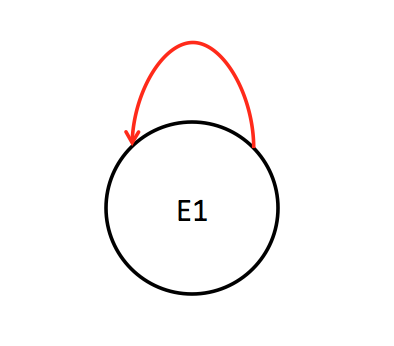
\includegraphics[scale=0.5]{selffeedback}
	\caption{\it Simple feedback loop with an entity supplying its input from its output.}
	\label{fig:exampleselffeedback}
\end{figure} 
Feedback loops can be encompass multiple entities, in Fig.~\ref{fig:exampletwofeedback} a feedback loop is shown that encloses two different entities. A output from $E2$ is passed to $E3$ which in turn creates a new input for $E2$, though $E2$ input is not directly its own output, it does depend upon it. 
\begin{figure}[H]
	\centering
	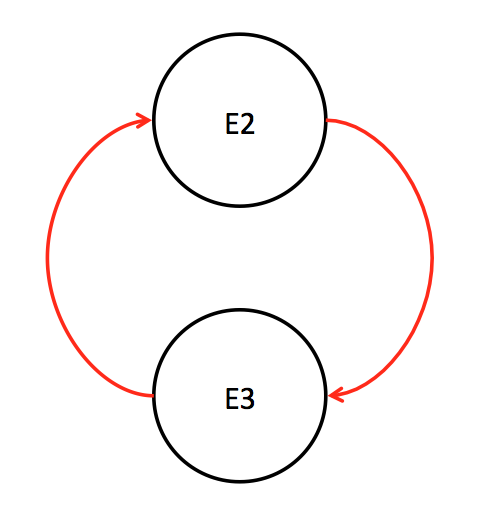
\includegraphics[scale=0.5]{twofeedback}
	\caption{\it Feedback loop between two entities, with each output being transformed by the other entity before becoming an input.}
	\label{fig:exampletwofeedback}
\end{figure} 
A loop such as the one in Fig.~\ref{fig:exampletwofeedback}, is only considered a feedback loop if information is passed through out the entire loop. If $E3$ produced a constant output, or an output that does not depend upon its input from $E2$, then this would not be a feedback loop as the new input to $E2$ does not depend on its output.\\
These example are very simple, feedback loops can be much more complex, encompassing any number of entities, each of whom can have very complex algorithms for transforming their inputs. Feedback loops can operate across time, meaning that an event in the past can eventually feedback to a present decision. For a feedback loop containing a large number of entities the time scale on which the feedback occurs can be come significantly large.\\
Though feedback loops are often assumed to be a negative property, some can be stabilising due to a benign effect.\\
Feedback loops can be present in a system in two ways, either they can be a constant fixture, called a static feedback loop, or they can form and change, called a dynamic feedback loop. A static feedback loop is present in the system from the start whether this is intentional and known, or unintentional and unknown to the members of the system. Dynamic feedback loops may not be present at the start and can form and change over time, with new entities joining or leaving them, allowing them to increase or decrease in size or effect, to split or merge, or to disappear.\\
Due to the potential complexity of feedback loops both in construction and in time, they can be difficult to detect, therefore methods are usually used to expose them. For static loops, forms of static analysis can be used such as, analysing initial setup, this is possible since the loops do not change through out time. Dynamic loops can be much harder to observe and analyses, an important aspect to detecting these loops is the interactions, messages sent between different entities within the system. Since the loops can evolve over time being able to track and analyse these messages over a time series is vitally important for the analysis of these loops, this time dependent analyse is called dynamic analyse.\\
Since feedback loops can be destabilising and damaging to the system in which they occur, there is interest in studying this emergence in the aim to prevent monetary loss and damage to the economy.\\
A notable form of emergence behaviour, due to feedback loops, that takes place within the electronic markets are flash crashes. A flash crash is an event during which time the trading price of a security drops very rapidly, becoming disconnected from its fundamental, before then recovering~\cite{rareeventflashcrash}. A particularly famous flash crash is that of 2010, in which the E-min S\&P 500 equity futures market dropped in price by more then 5\%, before rebound to close to its original price~\cite{SECreport_delays, rareeventflashcrash}. This whole process occurred very rapidly, lasting approximately thirty-six minutes and has been described as``one of the most turbulent periods in their history'' for the US financial markets~\cite{Impact_hft}.\\
Research done by Ref~\cite{DynamicCoupling_Chris, otherabmflash}, describes how the crash may have unfolded due to a feedback loop between High-Frequency Traders (HFTs), known as `hot-potato'' trading.\\
HFTs are a subset of algorithmic traders who normally participate in the market as arbitrageurs or market makers, they invest in ultra-high speed technology allowing them to detect, analyses and react to market condition in nanoseconds \cite{hftinformation1}. This means HFTs can trade huge quantities of assets in very short time frames, with some estimates stating that 10-40\% of all trades where initiated by them during 2016 \cite{hftmarketparticipation}.\\
The feedback loop of ``Hot Potato'' trading, is when inventory imbalance is repeatedly passed between HFTs market makers. A market maker is a trader who is required to have both a bid and a ask on the order book at all times, this means in theory that they are constantly buying and selling, a high frequency market maker as expected should be buying and selling very very often. Market makers make a profit from the spread and not long positions, hence they want to keep inventories low to avoid the market moving against them. To achieve this market makers have strict inventory limits that if they pass will cause them to go into what is know as a ``panic state'', during this state the trader will sell of an amount of its inventory to return back into its normal trading region. This inventory now sold by the market maker can be bought by another market maker causing them to in turn go into ``panic'' and sell, this process is ``Hot Potato'' trading and can in theory continue indefinitely~\cite{Elias_Paper}.\\
This constant selling and buying of inventory can artificially inflate the trading volume of the market, changing how many traders operate and potentially leading to a flash crash.\\
Flash crashes have occurred on a number of occasions and in a large selection of markets, with a more recent example being a crash of the cryptocurrency ethereum~\cite{cryptocrash}.


%%%%%%%%%%%%%%%%%%%%%%%%%%%%%%%%%%%%%%%%%%%%%%%%%%%%%%%%%
\subsection{Methods for Modelling Emergent Behaviour in Finance}
\begin{itemize}
  \item In Discrete time!
  \item Discuss different methods for modelling financial emergent behaviour (papers)
  \item compare where non-ABM and ABM papers are published (re-affirm need for this work)
  \item  What is a ABM 
\end{itemize}

\subsubsection{Recurrences Relations} 

\begin{itemize}
  \item Say that there is an alternative modelling technique which doesn't share the same problems 
  \item Introduce Recurrence Relations, what they are etc 
  \item Show and describe them, to a level that any one should be able to understand what they are 
  \item talk about emergence in them
  \item Show why loops and emergence are not necessarily bad or hard wired obviously into the system
  \item Say their benefits and down sides  \begin{itemize}
  \item can't follow messages in a system
  \item can view history of states 
  \item are well accepted 
  \item can have a formal definition 
\end{itemize}
\end{itemize}

Recurrence relations connect a discrete set of elements in sequence, these elements are normally either numbers or functions, they can be used to define these sequences of produce the elements in them. They can be seen as equations that give the next term in a sequence based on the previous term or terms, hence defining said sequence. Recurrence relations are often used to define coefficients in series expansions, moments of weight functions, and members of families of special functions~\cite{recurrelationbook}.\\
The most simplistic form of a recurrence relation is one where the next term depends only on the immediately preceding term. If the $n^{th}$ element in the sequence is defined as  $x_{n}$, then this recurrence relation can be written as,    
\begin{equation}
x_{n+1} = f(x_{n}),
\end{equation}
where $f()$ is a function that calculates the next term based on the previous one. A recurrence relation does not just have to depend on its immediate previous term and can depend on any number of terms further back in the sequences, for example a recurrence relation depending on terms from two and three steps before can be written as, 
\begin{equation}
x_{n+1} = f(x_{n-1}, x_{n-2}),
\end{equation}
with $f()$ now taking two inputs to produce the new term in the sequence~\cite{recurrealtionwebpage}.\\
Recurrence relations can also be used to define a sequence through time, in the simplest case the enumerate $n$, can be set to represent time $t$, this is applicable to discrete time as it requires set steps between the different times. Just as in the previous examples, the simplest recurrence relation is,  
\begin{equation}
x_{t+1} = f(x_{t}),
\end{equation}
where $x_{t}$ is the term at time $t$ and $f()$ gives the term at $t+1$ based on the term at $t$. Again this can be expanded to include terms from a number of previous time steps, allowing the memory of the sequence to be shown.\\  
A recurrences relation for defining a sequences may as well as depending upon previous terms, also depend upon some parameter, $\alpha$, this would give, in its simplest case, 
\begin{equation}
x_{n+1} = f(x_{n}; \alpha).
\end{equation}
The next term in the sequence may not only depend on previous terms within its own sequence and paramters, it can also be conditional on another sequence. For example one sequence through out time, $x$, may depend on another sequence through out time, $y$, a simple recurrence relation for this could be,
\begin{equation}
x_{t+1} = f(x_{t}, y_{t}),
\end{equation}
with the sequence for $y$ possibly depending on its own recurrence relation. The sequence for $x$ may not even directly depend on its own sequence and could solely depend on $y$, 
\begin{equation}
x_{t+1} = f(y_{t}).
\end{equation}
Though it could also indirectly depend on its self, if $y$ was defined by a recurrence relation depending on $x$, such as, 
\begin{equation}
y_{t+1} = f(x_{t}).
\end{equation}
These cross sequence associations allow for complex interactions to be represented as time series defined by recurrence relations, this is a method which can be applied to agent-based modelling.\\
Reference~\cite{econmistsnoabm} showed how an agent-based model looking at the microstructure of the financial markets, can be exhibited in the form of recurrence relations. In their approach each agent with in an $n$ agent model is considered to be well described by a state variable, $x_{i, t}$. The state variable describes the agent at each time step, where $i$ is the identity of the agent $(i \in 1,2,....,n)$, and $t$ is the time step at which the agent is being described, i.e. $x_{1,5}$ describes the first agent at the fifth time step. These state variables are defined by the recurrence relation,     
\begin{equation} \label{eq:notimedelayrecur}
x_{i, t+1} = f_{i}(x_{i, t}, x_{-i,t}; \alpha_{i}),
\end{equation}
where $f_{i}()$ is a function unique to agent $i$, that can take the state of the agent at the previous time step, $x_{i, t}$, the state of any other agent at the previous time step, $x_{-i, t}$\footnote{The $-i$ is used to refer to all other agents in the system. So if $i=1$, $-i$ refers to agents $2,3,4,....,n$, for an $n$ agent system.}, and a bespoke parameter $\alpha_{i}$.\\
This method works by describing each agent as a sequence of state variables, these sequences are then interlinked by having dependencies to each other, allowing both the agents and their interactions to be represented. A simple example of this could be two agents, $x_{1}$ and $x_{2}$, that are coupled to each other and only depend on the others value at the previous time step and a parameter, represented by the recurrence relations,     
\begin{equation}
x_{1, t+1} = f_{1}(x_{2,t}; \alpha_{1}),
\end{equation}
\begin{equation}
x_{2, t+1} = f_{2}(x_{1,t}; \alpha_{2}).
\end{equation}
This formulation only shows relationships to the previous time steps, however information delays can be added to the system by allowing the recurrence relations to have a longer memory. A recurrence relation that uses a state variable from three time steps ago, could be considered to have a time delay of three time steps in receiving this information. The generalisation of the model needed to allow for this, is a recurrence relation of the form, 
\begin{equation}
x_{i, t+1} = f_{i}(x_{i, t}, x_{i, -t} x_{-i,t}, x_{-i, -t}; \alpha_{i}).
\end{equation}
This is similar to Eq.~\ref{eq:notimedelayrecur} but contains two new terms $x_{i, -t}$ and $x_{-i, -t}$, these terms are used to refer to any time steps before the previous one, time $t$. This more general equation can now reference any state variable from any previous time, from any agent, as well as its bespoke parameter, to compute the next term in its sequence.\\  
This models can be solved for macro-level properties by iteratively solving each state variable, $x_{i, t}$, given some initial conditions. This method of assessing the model gives it a formal definition, and one that is accessible by a larger range of experts then classic agent-based models. Recurrence relations in a number of forms are commonly used in economics and finance and hence are familiar and relatable to economists, this makes them a far more effective tool for describing models to these domain experts then agent-based models.\\
This iterative method for solving the equations makes any dependencies between systems apparent, as if $x_{2, t}$ is present in the definition of $x_{1, t+1}$, one can say that $x_{1,t+1}$ depends on $x_{2,t}$. This transparency of dependencies makes this formulation amenable to static analysis, allowing the recurrence relations to be investigated to return their static dependencies.\\
Although all recurrence relations will contain some form of recursive, since this is an intrinsic property, this will not necessarily be negative or destabilising. For example a dependency on a state at a previous time step may not be destabilising to the system, however the reverse would be a case where the state variable at $t+1$ depended on its self, this would be a destabilising loop. Static analysis hence could be used to detect hard-wired destabilising loops, such as the one just mentioned.\\
Static analyse of the system can become difficult when the functions $f_{i}()$ contain conditional statements relating to their inputs, this can cause inputs not to be used at certain times hence meaning dependencies will not be as obvious as simply the inputs given, this is a problem of determining wether a function will necessarily evaluate all its arguments~\cite{willevaluteargsa}.\\
Though through static analysis recurrence relations can be used to view the history of the state variables of a single agent, however the history of messages between pairs of agents is not easily detectable with static analysis. The interaction history is found through dynamic analysis which is not well suited to recurrence relations, as they lack a clear ability to follow the passing of messages within the system.   


\subsubsection{Agent-Based Models}
There are a number of different techniques to model emergent behaviour in complex systems, one popular method is agent-based modelling. Agent-based modelling can be considered more of a mind set then a rigid methodology, this involves describing the system in question in terms of its components and then allowing these to interact. Agent-based models allow a system to be described naturally and are hence the canonical approach to modelling emergent phenomena. This method is a bottom up approach, allowing for each component of the system, agent of the model, to be created to a relevant degree of abstraction~\cite{abmhumsystems}.\\
Agent-based models have been used to model a wide range of emergent behaviour including in the financial markets, examples of this are, noise traders~\cite{abmnoisetraders}, herding among traders~\cite{abmherding}, and fundamentalists~\cite{abmfundemetilists}.

\subsubsection{Review of Literature on Financial Model} \label{litreviewofabmrr}
%compare abm and non abm of finacial markets and say that ecomists publish different papers 


\begin{itemize}
  \item Compare papers on RR and ABM and show that RR are used in finance papers more then ABM and hence the need for my project 
\end{itemize}

%RR
%https://link.springer.com/chapter/10.1007/978-3-642-46938-1_3 (book)
%https://books.google.co.uk/books?hl=en&lr=&id=o-clBQAAQBAJ&oi=fnd&pg=PA1&dq=recurrence+relations+finance+modelling&ots=v2yOVKquNP&sig=i0q6iZq3FHx_HEtvI4fsCQfmLD4#v=onepage&q=recurrence%20relations&f=false (book)
%https://books.google.co.uk/books?hl=en&lr=&id=7iGsCQAAQBAJ&oi=fnd&pg=PA185&dq=recurrence+relations+finance+modelling&ots=SPbejTEzwk&sig=qzu1gMUBiMCUtAFq1TSbP7YPKEc#v=onepage&q=recurrence&f=false (book)
%https://link.springer.com/chapter/10.1007%2F978-3-540-71297-8_41?LI=true (paper)
%http://www.jstor.org/stable/3481708?seq=1#page_scan_tab_contents (paper)
%https://www.researchgate.net/profile/Thomas_Mikosch/publication/2703398_Sample_ACF_of_Multivariate_Stochastic_Recurrence_Equations_With_Application_to_GARCH/links/54255bc90cf26120b7ac91db.pdf (paper draft)
%http://www.annualreviews.org/doi/abs/10.1146/annurev.economics.050708.142940 (paper)
%http://www.sciencedirect.com/science/article/pii/S0362546X97002356 (paper)
%http://www.sciencedirect.com/science/article/pii/S157400210502023X (paper)
%https://search.proquest.com/openview/f6cf1c4d1288dc7c9c2f34b31ab058e4/1?pq-origsite=gscholar&cbl=18750&diss=y (phd)
%



%%%%%%%%%%%%%%%%%%%%%%%%%%%%%%%%%%%%%%%%%%%%%%%%%%%%%%%%%
\subsection{InterDyne} \label{InterDyne_section}
\begin{itemize}
  \item Introduce InterDyne as the ABM which will be used here 
  \item Give a brief description of InterDyne 
  \item Say that we are using it because it is designed to investigate finance etc
  \item
\end{itemize}



%describe interdyne in a lt of detail so that the conversion later makes more sense, use diagrams
%rewrite a lot of this section to feel better 




InterDyne is bespoke simulator created by Clack and his research team at UCL~\cite{Chris_webPage}, it is a general-purpose simulator for exploring emergent behaviour and interaction dynamics within complex systems.\\
InterDyne design is that of an agent-based model interacting via a harness. This creates a structure of individual autonomous agents who interact through messages sent to one another.\\ 
Similar to other agent-based models InterDyne operates in discrete-time rather then continuous time. These quantised time chunks which move the simulation forward can be left with out proper definition, simply having operations defined in a number of time steps, or they can be equated to a real time usually with the smallest time gap needed be a single time step and then all other timings being integer multiples of this. This discrete time is most important to message passing, meaning messages between agents are only sent on a integer time step.\\ 
Massages in InterDyne are just small packets of data, such as a series of numbers.  Agents can only communicate via these messages, meaning that any emergent behaviour observed, that is not directly due to one agent, must be caused by linking of agents mediated by these messages. An agent can send private messages that are only received by a single other agents, one-to-one messages, or can send broadcast messages received by a number of agents, one-to-many messages. To facilitate this a communication topology can be made for InterDyne, this is done in the form of a directed graph determining which agents can communicate with each other. Due to the directional nature of these messages this topology could allow an agent to send messages to another but not be able to receive messages from that same agent. Messages have a defined order to them, an agent will, unless otherwise instructed, always process messages in the order in which they arrive. To change the order in which messages arrive delays can be added to communication paths between agents, this can be a static delay which always applies to messages sent from one agent to another, meaning this will arrive a set number of time steps later. Or a more complex dynamic delay, which is achieved by using another agent to mediate the passing of these messages delaying by an amount decided on in some internal logic. All messages in InterDyne are passed through a harness, this does not alter the messages or delay them\footnote{Unless instructed to using the static delay.}, but does store the messages and their order which can be used in post analyse.\\         
Each of the agents within an InterDyne simulation can be completely unique and modelled to different levels of complexity, as is the case with most agent-based models, allowing system components to be created to the level needed for the required experiment. As a whole InterDyne simulations are deterministic, repeated experiments will return identical results. However non-determinism can be added via the agents, making some part of an agent stochastic will lead to repeated experiments on the whole returning different results. A pseudo-random element can also be added by instructing InterDyne to randomly sort the message order for any agent receiving multiple messages in one time step. This is only pseudo-random as, as long as the same seed is used each run of the simulation will order the rearranged messages in the same way.\\
InterDyne is created to be particularly amenable to dynamic analyses of its simulations, this is achieved in part by all messages being sent via the harness allowing them to be stored in order.     


\subsubsection{Applicability to Finance} \label{applicabilut_to_finance}
%make sure I dont repeat stuff from the introduction 
%describe how a large order can cause a flash crash
%describe how high frequcey can cause that 

\begin{itemize}
  \item Explain the flash crash and that InterDyne is made to model it
  \item Explain how InterDyne is suited to modelling the flash crash 
  \item this should be a shortish section as it is not completely relevant (probably lose subheadings) 
\end{itemize}

Though InterDyne is a general purpose simulator, its main use thus far has been the exploration of financial markets. In particular InterDyne has been used to explore ``Flash Crash'' of 2010, during which market prices and rational valuations became disconnected, with some stocks trading as low as a penny per share, this lead to frenzied trading and irrational prices which spread between markets causing a massive price crash~\cite{SECreport_delays}. This event lasted around 36 minutes and has been described as``one of the most turbulent periods in their history'' for the US financial markets~\cite{Impact_hft}.\\
The hypotheses for this crash which InterDyne exists to investigate, is that this crash is an emergent phenomenon caused by the interaction between High Frequency Traders (HFTs) within the market.\\
HFTs are a subset of algorithmic traders who normally participate in the market as arbitrageurs or market makers, they invest in ultra-high speed technology allowing them to detect, analyses and react to market condition in nanoseconds \cite{hftinformation1}. This means HFTs can trade huge quantities of assets in very short time frames, with some estimates stating that 10-40\% of all trades where initiated by them during 2016 \cite{hftmarketparticipation}.\\
The type of interaction between these traders suggested to have caused the crash is ``Hot Potato'' trading, this is when inventory imbalance is repeatedly passed between HFTs market makers. A market maker is a trader who is required to have both a bid and a ask on the order book at all times, this means in theory that they are constantly buying and selling, a high frequency market maker as expected should be buying and selling very very often. Market makers make a profit from the spread and not long positions, hence they want to keep inventories low to avoid the market moving against them. To achieve this market makers have strict inventory limits that if they pass will cause them to go into what is know as a ``panic state'', during this state the trader will sell of an amount of its inventory to return back into its normal trading region. This inventory now solid by the market maker can be bought by another market maker causing them to in turn go into ``panic'' and sell, this process is ``Hot Potato'' trading and can in theory continue indefinitely~\cite{Elias_Paper}.\\
``Hot Potato'' trading was observed in the market during the ``Flash Crash''~\cite{SECreport_delays}, this is thought to have been caused by a combination of an initial large sell order by a mutual fund and delays in communication between HFTs maker makers and the exchange on which they were operating on, causing them to buy more inventory then they wanted and go into a ``panic state'' and hence a ``Hot Potato'' feedback loop.\\       %rewrite this a bit, add more detail
This section explains in more detail this hypotheses and how InterDyne is set up to investigate it.  

\paragraph{Deterministic}
The deterministic nature of InterDyne allows for experiments to be run multiple times with the same result always returned, this allows for changes to the experiment setup to be investigated. For example changing the number of traders in the market and comparing this to a previous run allows for an investigation into how many traders are required for emergent behaviour to be observed.\\
This becomes particularly interesting when comparing the interactions between market makers to that of the n-body problem, like with this problem one could expect emergent behaviour might occur to some extent in a large group of market makers, however the question of wether the emergence persists in a comparable market to the three-body problem and how this compares to a larger market can be investigated.   


\paragraph{Message Delays}
Allowing the delaying of messages is intrinsically important to the investigation of the hypotheses since the existence of delays is proposed as one of the main aspects in the ``Hot Potato'' trading that occurred. Delays exist between all aspects of the market which can account for the processing time of the different elements and the transmission time of messages between them. Some of these delays will be static but it has been preposed that the delays related to the exchange actually increased during the crashing, further worsening the situation~\cite{SECreport_delays}.\\
Static delays in built in InterDyne can be used to investigate the crash to see if it can occur without the need for dynamically varying delays. Dynamic delays created with agents can then be used to further investigate the events that occurred during the crash, allowing a situation to be set up where as more messages are sent to and from the exchange its delays increase.  Asymmetric delays can be specified between two agents allowing further investigation into the environment in which a crash is mostly likely to occur and how delays could be altered to reduce this out come. 

\paragraph{Message Passing}
To observe the decided system level behaviour, a flash crash, two different methods can be use; the behaviour can be encoded into the program forcing it occur at a system level, or the system can be setup to allow the behaviour to emerge at the system level. For a true understanding of emegernt behaviour the latter approach is more relevant, this requires the different agents within the simulation to be able to communicate directly with one another. In modelling the financial market these communications are in the form of messages sent between different entities, for example a trader could send a message to an exchange detailing a limit order they wish to issue and an exchange could send back a message containing a confirmation of this order.\\
These messages allow interaction dynamics to occur within the simulation and hence for emergent behaviour derived from interaction dynamics to naturally present within the system. 




\paragraph{Storing Messages}
Due to the nature of emegernt behaviour being usually unexpected, it can be very difficult to to deduce what low level structures and operations gave rise to this system level phenomenon. This is especially true when modelling a financial system that has a large number of interacting agents all sending and receiving messages, some of which can be delayed changing their expected order of arrival. The delays in the system have been suggested to have influenced the emergence of behaviour within the system, hence in investigating these systems it is important to take into account not only message counter-parties but also message timings. InterDyne facilitates post simulation analyse into this by being able to produce a trace for all time steps of the full information of; messages sent by any agent, messages received by any agent and messages being delayed before being delayed to an agent.          

  
\paragraph{Discrete Time}
Though it is easy to assume that the financial markets operate in continuous time this is in fact not always the case. For electronic markets that trade through an exchange their time is set by the exchange, orders are not processed and messages are not sent back till the exchange decides to do so. These electronic exchanges them selfs operate in discrete time, this is unavoidable and is a product of the systems being run on computers, a computer runs based on an internal clock that ticks in discrete intervals based on a change in a square-wave oscillating voltage. This change in voltage is so fast that to a human it seems continuous, however HFTs operate themselves at such high speeds that the system clock time gaps are comparable and hence need to be considered. Therefore models simulating HFTs interactions to this detail must take account of this discrete time, hence InterDynes discrete time nature is a good match to model HFTs interactions.     
     

\paragraph{Message Ordering}
The order in which messages are processed can be very important, for an exchange, for example, it can change whose limit order has priority at a given price and whose market order executes the lowest prices. Changing these factors can make or break feedback loops within the system, meaning if message ordering is not properly dealt with the correct emegernt behaviour may not be observed. Hence InterDyne stores messages in the order they are received by an agent, taking into account delays to the messages. This however can not be done when multiple messages are received at the same time step, due to the nature of discrete time there is no way for the agents to know which message arrived first, therefore two options are presented by InterDyne; messages are ordered according to their agent identifier %say what this is in a foot note?
or messages are randomised and executed in the  emerging order. This randomisation is handled in the same manner every run of the simulation \footnote{This can be changed using a new seed if so desired} hence resulting in the same order and therefore not effecting the deterministic nature of the experiment.  


\paragraph{Agents}
%expand this section

A benefit of agent based models of other alternatives is the ability to encode agents as unique traders instead of having to model the general behaviour of a number of traders. This allows for unique behaviour of varying complexity to be given to different agents, facilitating experimentation with different trading strategies, allowing different questions to be investigated, such as, does a trading strategy need to be complex for emergence to be observed? 




\subsubsection{InterDyne Detail Operation}

\begin{itemize}
  \item Explain in detail InterDynes operation
  \item The detail level here should be enough that the conversion later makes sense 
  \item Diagram of InterDynes operation 
  \item Introduce the harness and agents, as well as their types 
\end{itemize}

InterDyne is an agent-based model simulator written in the Haskell language. An InterDyne simulations structure, shown in Fig.~\ref{fig:harness_setupfigure}, consistent of a number of independent agents, sending messages to a ``Simulation Harness'', this harness then (i) sends these messages to the relevant counter party or parties \footnote{In the case of broadcast messages}, (ii) saves these messages to a trace file.   
\begin{figure}[H]
	\centering
	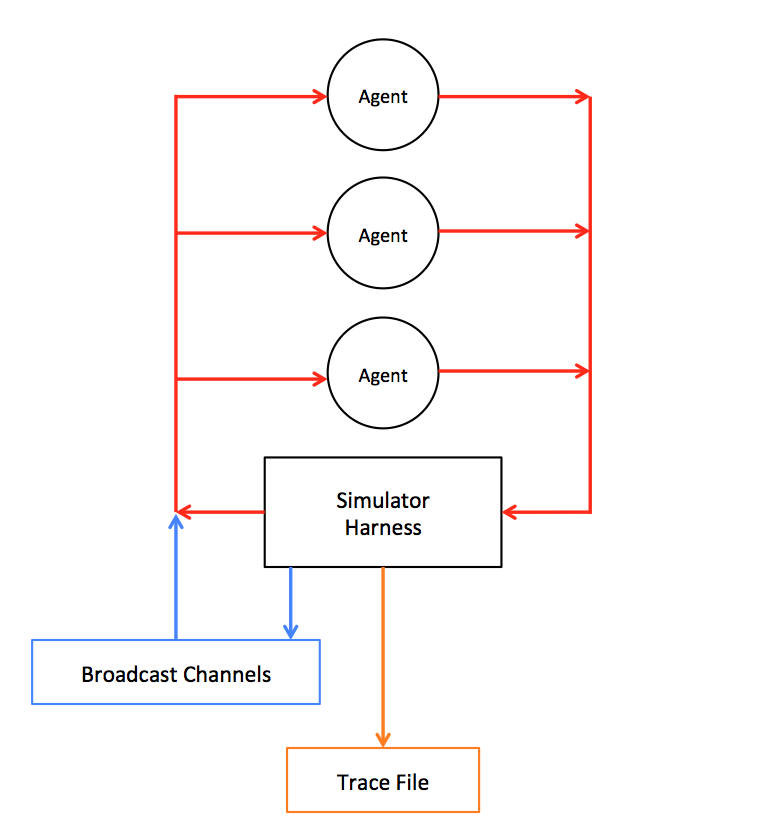
\includegraphics[scale=0.5]{harness_setup}
	\caption{\it Structure of an InterDyne simulation containing three agents.}
	\label{fig:harness_setupfigure}
\end{figure} 
%%%%%%use diagram from user manual
By set up each agent is required to both consume and produce a message at every time step, this is done by sending each agent a potentially-infinite list of messages and requiring it to create a potentially-infinite list of messages. The inbound list contains every message the agent will receive through out the entire simulation, ordered by time, and the outbound list contains every message the agent will ever send, order by time. This is possible due to lazy evaluation of the language that InterDyne is written in, This means that only messages being used are evaluated. Since no agent should attempted to use a message from the future \footnote{If they do an error will be thrown.}, only messages that have been created so far are read.\\
Since the set up of these list requires an element for every time step and an agent my not need to send a message during a time step, empty messages can be sent, this will result in an agent either receiving or sending an empty list. It may be the case in a simulation that an agent could be generating empty messages by mistake, to differentiate between a message empty by mistake or by choice, a message can be created containing ''Hiaton`` demonstrating that it is empty by choice.\\   
A InterDyne simulation once created can be run by executing the ''sim`` function with relevant arguments, this function has a type,      
\lstinputlisting[language=Haskell]{simplerunInterdyne.hs}
corresponding to, number of time steps, list of ``runtime arguments'', and a two tuple with the agents function and broadcast channels to which it is subscribed.\\
Agents within a simulation are defined by ID numbers, with the first agent having ID=1, followed by the second agent with ID=2,  ID=0 is used to represent the ``simulator harness''. These ID numbers are used to specify which agents messages are coming from and going to. This however can be difficult to keep track of within large experiments for the experimenter, therefore InterDyne allows for agents to be referred to by a name. This example shows InterDyne being run with the use of names for identification:     
\lstinputlisting[language=Haskell]{fullunInterdyne.hs}
This simulation will run for 60 time steps, with three agents subscribed to a number of broadcast channels, for example the third agent is subscribed to channel 2 and 3. There is a single run time argument convert, that can convert an ID to a name and a name to an ID. This is a simplistic call of the function sim, but shows how an experiment run could be setup and executed.\\   
In the example one can notice that the agents called all were to referred to as wrappers, this is because agents in InterDyne are typically, though not necessarily, written in two sections; ``wrapper'' and ``logic'' functions. The ``wrapper'' function, called in the example, can be thought of as the true agent, it handles message receiving and sending, as well as updating the local state of the function, hence this function is the one that interacts with the other agents and the harness. The ``logic'' function rests inside the ``wrapper'' function and computes the messages to be sent, hence this contains the functionality of the agent. An example of a ``wrapper'' function containing a ``logic'' function is shown here:
\lstinputlisting[language=Haskell]{complexagentwrapper.hs}
This agent will output a list containing message m, which is the output of the ``logic'' function for that given time period based on the received messages. The wrapper is a recursive function with each recursion being a new time step. It takes as inputs, st the local stat variable, args the run time arguments, a list of all messages to it, and its ID.  The list of messages has a three tuple for each time, containing the current time, list of all messages sent to the agent directly, and a list of all messages sent to the agent from broadcast channels.\\ 
InterDyne supports a wide range of messages in an array of complexities, to allow for a variety of interactions to take place. Messages, which are either one-to-one or broadcast, must all contain a pair of integers which represent the sending agents ID and the receiving agent or broadcast channels ID, the rest of the message depends on the type of message being sent. For example one could send a one-to-one message containing a list of (key, value) pairs, 
\lstinputlisting[language=Haskell]{message_simple.hs}
or a message carrying a string, 
\lstinputlisting[language=Haskell]{message_data.hs}
Broadcast messages content is defined by a broad type, which defined further within its type definition, 
\lstinputlisting[language=Haskell]{message_broadcast.hs}
As previously stated ID=0 represents the harness, messages sent to this ID are printed to an output file, output is also achieved in InterDyne by storing all messages of type Datamessage, which are saved to a different file then those sent to ID=0.\\  
As mentioned earlier InterDyne allows for both a topology of allowed interactions and delays along interaction paths to be defined. This can be done by passing two runtime arguments to the ``sim'' function \footnote{Both the arguments must be given.}, (i) a function that when given two agent IDs will return a delay for the interaction between them in time steps, and (ii) the maximum delay that returned by this function, i.e. the maximum delay present in the system. The previous example expanded with delays is shown here: 
\lstinputlisting[language=Haskell]{interdynewithdelays.hs}
Once delays have been specified in this manner all messages, one-to-one and broadcast, are delayed by the stated amounts between the defined agents. Dynamic delays are not shown here, but are achieved with use of another agent acting as a go between \cite{Chris_webPage}. 
 






%\subsection{Examples}


%Day and Huang [Day, R. And Huang, W., ?Bulls, Bears and Market Sheep?, Jourmal of Economic Behaviour and Organisation, 1990] for example have demonstrated how interactions between two simple but different trading strategies and a market-maker can cause complex emergent features of stock market prices such as alternating periods of rising (?bull market?) and falling (?bear market?) with sudden switching between the two at irregular intervals. Further, Lyons [Lyons, R.K. ?A Simultaneous Trade Model of the Foreign Exchange Hot Potato?, Journal of International Economics 42 (1997) 275?298] has shown how a feedback loop can emerge between foreign exchange dealers, causing them to repeatedly transfer inventory between themselves.  Yet these are simple models of interaction.  Our aim is to develop a framework for modelling and analysing more complex emergent behaviour that arises from the dynamics of interaction, and in the context of our case study to analyse behaviour that may increase risk to the stability of the financial markets.

%\subsubsection{Hot Potato} 
%what is hot potato
%fx market

%this is a dynamic feedback loop
%how is it caused 
%when has it happened 

%what is a hft (probably need a subsectuion on this)
	%how do they work
	%what do they do
	%market makers
	%inventory limits
	%why do simple versions of them still work

%This feedback effect has been shown, in the InterDyne simulator, to create instabilities in market prices and even lead to crashes~\cite{DynamicCoupling_Chris}.   






%\subsubsection{Flash Crash}
%lob version of hot potato
 
%what is the flash crash
%when have they happned 
%other theories to why they happen?
%what we think causes them
	%emergence from feedback loops in hfts
%why they are important
%A flash crash is defined as a quick drop and then recovery in securities prices, with the most infamous  crash occurring on the 6th of May 2010 and lasting for around 20 minutes in which time almost one trillion dollars of market value was lost~\cite{Vikram_Paper}.\\
%There is no consensus on the exact cause of the flash crash, however a number of theories exist. The theory that InterDyne models is that the flash crash was caused by an interaction effect between High Frequency Trader Market Makers, known as the hot potato effect~\cite{Elias_Paper}. 



%There are numerous examples of emergent behaviour in the financial markets caused by interaction dynamics within the SoS, here we will look at how the US markets ?Flash Crash? of May 6th 2010 [CFTC-SEC, 2010. ?Findings regarding the market events of May 6, 2010?] may have been caused by these interaction dynamics. 
%The term ?Flash Crash? here is used to describe an event within a financial market where the price of commodities plummets extremely quickly before rapidly rebounding. This kind of behaviour tends to go hand and hand with commodities becoming disconnected from their fundamental value, such as stocks for companies trading at far lower prices despite the fact that mothering has change about the company in question.
%The crash in question occurred within the E-mini S&P 500 market, EXPLAIN WHAT THIS MARKET IS, lasting approximately thirty minutes [REF] with the prices for some stocks falling as low as a penny a share [REF].
%FIGURE OF FLASH CRASH??? 
%There has been a large amount of speculation about the cause of this crash with blame levelled at a large sale by a mutual fund, spoofing by a independent trader and the hot potato effect between High Frequency Traders (HFTs), it is the later that we are interested in here.
%HFTs are algorithmic traders who use equipment that allows them to operate at nanosecond speeds [REF], this means huge amounts of trading can occur between HFTs before a human can process what has happened.  Not sure how to phrase this but want to say that a lot can go wrong before a human realises 
%HFTs often operate as a Market Maker, these are entities that both buy and sell with the market under a set of rules, such as having to always have a bid and ask on the order book, they are then rewarded by having discounts applied to their trades. Market Makers make their profit of the difference in price between buying and selling assets and not of the fluctuation in price of an asset over time. They would not buy assets with the aim of selling them in a few days as they think the price would increase, instead they buy and sell the assets normally within a few milliseconds. As such having a large inventory of any asset is considered to be risky by the Market Maker and they will normally have thresholds on their stock, if these thresholds are passed, they have more stock then they want, they will enter an aggressive selling phase, quickly reducing their stock back below their thresholds. When this occurs the HFT is said to be in a panic state, the inventory at which this panic state occurs can be dynamic, changing demanding on the perceived risk within the market and how the Market Maker is trying to preform. 
%Since HFTs can place orders so quickly and make their profit of buying and selling they will normally have orders near or at the touch, the best bid and ask. This means that if you trade on the market you are likely to execute your trade with a market maker first SAY WHAT PERCENTAGE OF TRADES THE MARKET MAKERS ARE RESPONSIBLE FOR [REF]. This means that if a Market Maker goes into panic it is likely to sell its stock to another Market Maker; this creates links between the Market Makers as they will buy and sell to each other during panic states.  
%There are a number of methods used for exiting a panic state, enough inventory can be solid to bring the Market Maker back to exactly its limit, more can be solid to bring it below its limit by a set amount or all the inventory can be solid to reduce the risk to the Market Maker to zero. Each of these different options changes how much stock will be passed on to another Market Maker during the panic state.
%The question then arises, what happens if the Market Maker who buys this excesses stock is already near its inventory limit? In this case the receiving Market Maker can also enter panic, causing it to sell its inventory back to the market. As can be imagined in the right market conditions, this inventory can be picked up by another Market Maker who is also close to their limit and hence the processes can continue. If this inventory passing between the Market Makers forms a feed bank loop, where the initial Market Maker receives the stock again before selling it on for a second time, it can be said that ?Hot Potato? effect is occurring, this is simply the processes of passing inventory around traders in a loop.    
%There are a number of reason a Market Maker could be near its limits or go into panic, it could be already near its limits and then be forced to buy more inventory by the exchange rules. It could dynamically shift its risk limits changing its inventory boundaries causing it to go into panic or at least approach its limits or it could make a number of assumptions about its sell orders which may be incorrect. 
%A reason assumption are made is because of time delays with in the system. 





%%%%%%%%%%%%%%%%%%%%%%%%%%%%%%%%%%%%%%%%%%%%%%%%%%%%%%%%%%%%%%%%%%%%%%%%%%%%%%%%%%%%%%%%%%%%%%%%%%%%%%%%%%%%%%%%%%
\section {Description and Analysis of the Problem} \label{despriptionandanalysproblem}
\begin{itemize}
  \item Introduce the idea that agent based models and InterDyne have flaws
  \item Say that though they have been used for experiments their results are not always accepted 
  \item Explain the layout of this section 
\end{itemize}


%desciption an analysis
%what is the problem, why is it important, why is difficult
%in intro and alaysis state how different the interdyne and recurrance relations are  
Though InterDyne is a functional simulation platform and has been used to run a number of experiments, most notably in Ref.~\cite{DynamicCoupling_Chris} where a model was presented showing a flash crash caused by interaction dynamics, it possesses a concern when discussing these results, especially to non-experts in computational modelling.\\
This section will discuss the main draw backs of InterDyne and a method for countering them.  



%%%%%%%%%%%%%%%%%%%%%%%%%%%%%%%%%%%%%%%%%%%%%%%%%%%%%%%%%
\subsection{Why Agent-Based Models Are Not Enough} \label{Iinterdynenotenough}

\begin{itemize}
  \item Say why agent based model and Interdyne are not always accepted
  \item list the down side of agent based models \begin{itemize}
  \item inverse function problem
  \item tracking parameter effects
  \item model as a whole lacking formal definition 
\end{itemize}
  \item Explain this issues in detail 
  \item Mention positive of ABM, such as easier to track messages and hence emergence and good for dynamic analysis 
\end{itemize}

As already mentioned InterDyne is an agent-based model and hence possesses the same limitations as do other models of this type. A number of these limitations are of particular concern to economists, making agent-based models and their results not commonly accepted by them~\cite{econmistsnoabm, lob_noecomimists}. The most significant limitations  with this models are:
 \begin{enumerate}
  \item Producing high-level behaviour or emergent behaviour from a set of base rules, only shows that those create it and does not show that those are the only rules that could exhibit this behaviour. This is often referred to as the inverse function problem.
  \item Tracking the affect of an input parameter on the output of the agent-based model can be very difficult, and parameter-estimation may be done in a fashion that will not represent all of the possible outcomes of the model. 
  \item Despite each agent within a simulation being fully specified the model as a whole will lack a formal definition. 
\end{enumerate}
The first limitation is shared by man modelling techniques and is a by product of studying emergent behaviour, more then one scenario may lead to the same emergence. This limitation should be considered more as a consideration when analysing results from experimentation, it is generally speaking useful to find a set of conditions that lead to an emergent behaviour, but should be noted that it can not be said that it is the only one without further research.\\
The second limitation can be reduced by analysis of the sensitivity of the outcomes to parameter selections, this is shown in Ref.~\cite{econmistsnoabm}.\\
The third limitation is of particular interest, though the other limitations can lead to questions of the validity of findings from agent-based models, the understanding of the actual model and experiment being undertaken is hindered by this limitation. A resolution to this problem was put forward by Ref.~\cite{econmistsnoabm}, in which a formal definition of the specification of the an agent-based model was given in terms of a set of recurrence relations. This solution not only provides a formal definition of an agent-based model but also does so in a way which is relatable to non-programmers, such as economists.     



%%%%%%%%%%%%%%%%%%%%%%%%%%%%%%%%%%%%%%%%%%%%%%%%%%%%%%%%%
\subsection{Two Views Approach} \label{twoviewsapproach} 

\begin{itemize}
  \item What is Two-Views
  \item why have two-views: \begin{itemize}
  \item its a way of being able to look from two perspectives, good for hypotheses formalisation 
  \item an intro into ABM for economists
  \item can provide more faith in ABM 
  \item Communication tool between fields (science and economics)
\end{itemize}
  \item Difficulties in two-views: \begin{itemize}
  \item two paradigms are completely different
  \item Differences between function calls and messages
  \item name control, in a way that allows for a useful and tangible ABM
  \item Show problem as a whole despite splintering
\end{itemize}
  \item explain benefits and difficulties in detail 
\end{itemize}

As can be seen from the previous discussions neither agent-based models, in the form of InterDyne, or recurrence relations offer an optimal modelling technique whose results can be analysed to the level desired. With InterDyne suffering from a lack of a formal definition and difficulties for static analysis, and recurrence relations being unsuitable to preform dynamic analyses on. Looking at the benefits of the two techniques, InterDyne is well suited to dynamic analyses, and recurrence relations provided a formal definition and are appropriate for static analyses, one can see that they match each others draw backs.\\ 
Therefore a more ideal model, would be representable in both recurrence relations and as an agent-based model.  This model would be suited to both static analyses, while expressed as recurrence relations, and dynamic analyses, when in the form of an agent-based model. A model that can correctly transform between a set of recurrence relations and an agent-based model, would provide the agent-based model with a formal definition in the form of the recurrence relations. This method will be referred to as the two views approach, with recurrence relations, and agent-based modelling seen as two complementary views of the same system.\\
To create a model tool which will allow for the two views approach, three aspects most be covered, an agent-based model,the recurrence relations, and a convertor for transforming between them. The agent-based model as already been created in the form of InterDyne and as already discussed fulfils all the needed requirements for the systems being modelled. The latter two aspects however have not been previously produced and will be the focus of this paper.      

\subsubsection{Step-by-Step Transformations} \label{whyusestepbystep}
%a small literay review on why to use a step by step transformtion to go between the two vies 

%for literate review
%check if any one has done this before or anything similar 
%translating from RR to anything else 
%tralsing from anything to an agent based model 
%any one written anything on porcess fo program transformation by small steps, (lots in the late 80s), le brain phd theise (2000), desgined a programing langauge, approach he took to turn it into a functional langauge using step by step transoting (clover) 
%object flaw, paper 
%the clover rewrite rules, paper (this is the one i want)
%introducing clover and object oriented  functional langue, paper 


%for literate review
%compare abm and non abm of finacial markets and say that ecomists publish different papers 
%check if any one has done this before or anything similar 
%translating from RR to anything else 
%tralsing from anything to an agent based model 
%any one written anything on porcess fo program transformation by small steps, (lots in the late 80s), le brain phd theise (2000), desgined a programing langauge, approach he took to turn it into a functional langauge using step by step transoting (clover) 
%object flaw, paper 
%the clover rewrite rules, paper (this is the one i want)
%introducing clover and object oriented  functional langue, paper 

%EXPLAIN?? explain why a step-by-step processes should be taken refrencing other work using step by step transformations
%https://www.semanticscholar.org/paper/The-Clover-Rewrite-Rules-a-Translation-from-Oofp-t-Braine-Clack/4402741aa70e4cae37839f196b5741fd6b843428
%https://pdfs.semanticscholar.org/5b13/9a35dbc63e516dd51f2cd6672d2d7b5c21b6.pdf?_ga=2.246578180.1291348853.1500637404-583838121.1500637404




%%%%%%%%%%%%%%%%%%%%%%%%%%%%%%%%%%%%%%%%%%%%%%%%%%%%%%%%%%%%%%%%%%%%%%%%%%%%%%%%%%%%%%%%%%%%%%%%%%%%%%%%%%%%%%%%%%
\section{Bespoke Recurrence Relation Language}

\begin{itemize}
  \item Introduce this as the RR that are going to be used for the conversition
  \item why use a custom language? need to restrict the user enough to make the language comparable to Lambda calculus while maintaining all needed functionality, easiest to do this with own language, also need know full definition of language for parsing 
  \item what functionality does the language have? 
\end{itemize}


Recurrence relations are used across a wide range of disciplines and as such have many different forms of notation, since these recurrence relations are going to act as an import for the convertor program, having a wide range of possibly conflicting notations is not ideal. Therefore it was decided that a bespoke notation for the recurrence relation input should be used, this language will force recurrence relations to be written in a set form for input into the convertor.\\
In designing this language a few main considerations had to be taken into account:    
\begin{enumerate}
  \item The language needs to be able be both understood by and written by non-computer scientists, such as economists and mathematicians. 
  \item The language needs to be as simple as possible, to keep it easy to formally define and learn.
  \item The language still needs to contain enough functionality to fully specify the problems being modelled.
\end{enumerate}
The first consideration is taken into account by choosing the language to based in a more mathematical style then one that heavily relays on a computational style.%not sure about this sentence
The second and third consideration go hand in hand, requiring that the functionality of the language be as simple as possible while still allowing for the problem to be expressed. As such it is pertinent to decide what functionality is required by the language, this functionality is:      
\begin{itemize}
  \item The use of basic mathematical operations.
  \item The use of lists.
  \item The ability to call the head of a list. %hd
  \item The ability to call the tail of a list. %tl
  \item The ability to add to the head of a list. %:
  \item The ability to declare variables.  
  \item The ability to define a unique name for each recurrence relation.
  \item The ability to define a recurrence relation that uses inputs.
  \item The use of where blocks.
  \item The use of if else statements. 
  \item The ability to specify an entire experiment and initial conditions.  
\end{itemize}
It was decided that this language would be created by using an already existing coding language and reducing its functionality down to what was required. This resulted in the recurrence relation language being a simplified version of the Miranda language, Miranda was chosen as it is a functional language whose structure is similar to that of a set of mathematical equations, hence making it easier to adapt for use by non-domain experts.   


%%%%%%%%%%%%%%%%%%%%%%%%%%%%%%%%%%%%%%%%%%%%%%%%%%%%%%%%%
\subsection{Syntax}
%write this in a formal syntax as well BNF

\begin{itemize}
  \item show the formalised syntax of the language here   (neaten this up a lot)
  \item explain the syntax  
\end{itemize}


\begin{figure}[H]
	\centering
	\lstinputlisting[language=Miranda]{Syntax_Def.lit.m}
	\caption{\it Simple example of recurrence relations written in custom defined language.}
	\label{fig:parsetreecode}
\end{figure} 


%%%%%%%%%%%%%%%%%%%%%%%%%%%%%%%%%%%%%%%%%%%%%%%%%%%%%%%%%
\subsection{Rules of Use}
%any function can access any other fucntion within the same agent at the current time (or passed times) but any function in a different agent can only acess at earliest one time step ago.

\begin{itemize}
  \item Explain how to write something in this language and what the language can and cannot do in more detail 
\end{itemize}




%%%%%%%%%%%%%%%%%%%%%%%%%%%%%%%%%%%%%%%%%%%%%%%%%%%%%%%%%
\subsection{Example of Use}
%incude that t is a key word and needs to go at the begining of timevarying reccruance relations eg t1_inv t a b c = ..
%Syntax of the functionality, how do you write all the different elements 
%t is special means time 
%c_ is used as a way of dealing with names/custome types (can not call functions)
%varbiles are just that and cant call fucntions


\begin{itemize}
  \item Show and explain an example of the language (some explain that will be converted) 
\end{itemize}

Here the syntax for the above listed functionality will be explained, in ordered of listing.\\
Basic mathematical operations are allowed, plus $+$, minus $-$, times $*$, divide \textbackslash. The ability to make comments that will not be read is also allowed, a comment is started with ``\textbackslash\textbackslash'' and then the rest of the line is ignored.\\ 
The main method for storing and transferring information between recurrence relations will be in the form of lists, lists follow the same rules stipulated by the Miranda language. A list can be created by putting the elements in side ``[]'' and separating them with a comma, allowing lists to be written in forms similar to:
\lstinputlisting[language=Miranda]{exp_list_variations.m}
However all elements in these lists must be of the same type.\\
The head of a list will be extractable using the command $hd$, this will return the first element of a list, for example $hd$ called on the list $[1,2,3]$ would return $1$. Similarly the tail of a list can be called using $tl$, for example calling $tl$ on $[1,2,3]$ would return $3$.\\  
Elements can be added to a list using the command $:$, this can be applied in the form $4:[1,2,3] = [4,1,2,3]$.\\
Variables can be declared in the language, these are names that are attached to fixed values, and can be written in the form: 
\lstinputlisting[language=Miranda]{expl_varibles.m}
A variable name must state with the identifier $c\_$, this indicates that the object is a constant, this underscore is then followed by the unique name of the variable, an equals, and then the value to which the variable refers.\\   
A recurrence relation is defined in a similar way to a variable, but can take inputs and represents a function:
\lstinputlisting[language=Miranda]{expl_simplerecurrance.m}
The name must state with a identifier of what agent, $agent\_$, this recurrence relation belongs to, in this language all recurrence relations belong to an agent. A group of recurrence relations that belong to an agent will interact with each other but only have a single recurrence relation that interacts with a different agent, group of recurrence relations. After the agent identifier, the unique name of that recurrence relation within the agent is given, recurrence relations belonging to different agents may have the same name but with an agent the name must be unique. Then the inputs for this recurrence relation are given, there may be one or more inputs\footnote{A recurrence relation with no inputs is just a variable.} separated with a space between them. Then after the equals the function for the recurrence relation is give, this function may call on other recurrence relations.\\
A where block is used to define functions and variables unique to a certain recurrence relation, one can be written as follows:
\lstinputlisting[language=Miranda]{expl_whereblocks.m}
Inside a $where$ block which is identified by ${}$ any number of functions and variables can be defined, with each new one appearing on a new line.\\
This language facilitates the use of if else statements, this allows for different behaviour based on the inputs to the recurrence relation, this can be written in the form:
\lstinputlisting[language=Miranda]{expl_ifelse.m}
Using the command $myif$ declares that an if else statement is being used, then within brackets the condition for the if statement is given, this can use $<, >, \leq, \geq, =,$ etc. If this statement is true then the $then$ part of the statement is executed, if this is false the $else$ part is used.\\
 An experiment can be defined with initial conditions in the following way:
\lstinputlisting[language=Miranda]{exp_layout_gen.m}
The design of this is one where the $where$ block contains all the definitions for the recurrence relations in the experiment. Above this the $main$ defines an experiment to run, such as a recurrence relation that you want to iterate ten times. The initial conditions are defined above this, these can have multiple different values depending on an input parameter. At the top $run\_main$ gives a list of the $main$ with different values of $runnumber$ which corresponds to different values of the initial conditions.\\
 



%what the new language looks like 
%what each bit means
%what is allowed to be written
%how to write certain things
%how is it user friendly
%why this was choosen, for example easier to convert to lambda calcualse 

%\subsection{Examples}
%examples on how to use the grammar


\lstinputlisting[language=Miranda]{inv_code_simpleexample.m}

tuples exist but can not be used by the user 
%a very simple example on the use of the grammar
%\subsubsection{Complex Example}
%what I have actually done maybe?




%%%%%%%%%%%%%%%%%%%%%%%%%%%%%%%%%%%%%%%%%%%%%%%%%%%%%%%%%%%%%%%%%%%%%%%%%%%%%%%%%%%%%%%%%%%%%%%%%%%%%%%%%%%%%%%%%%
\section{Recurrence Relation to InterDyne Converter} 

\begin{itemize}
  \item Re say what the convertor is and what is meant to do
  \item Re say project scope and that here the converter is only being designed 
  \item say that is takes a step by step approach and why 
  \item why? so that the steps can be shown to be correctness preserving later more easily 
  \item say what the steps are going to be 
\end{itemize}

%defines the design of each step in the conversion between recurrance relations and interdyne 

%how I will create the two views
%what the converter is meant to do


%how would this work? correctness preserving transformation 

% Eventually, we would like to be able to express the System of Systems as a set of recurrence relations and then generate the agent-based model automatically; if this could be done in a way that preserves the semantics of the specification, then we would be confident that the static and dynamic analyses are being performed on models of the same System of Systems. 

This section details the design of the transformation from a set of recurrence relations written in the previously discussed custom language into an InterDyne simulation. This transformation processes  as been split into a number of smaller steps, with each step taking the expression of the system given by the previous step and modifying it to be closer to the InterDyne formalisation.\\
The transformation has been split into small steps to avoid any large jumps in logic between different representations. Jumps in logic can make it difficult to follow the transformation and more challenging to prove the correctness of the transformation.\\
The aim of this section is to show the design of each of these transformative steps, and not to implement them into code or prove their correctness, however in some case the code may also be shown.\\
To assist in the explanation of the transformation a simple example will be used through out this section Recurrence Relation Example 1 (RRE1), this example is shown in Fig.~\ref{fig:rre1}. 
\begin{figure}[H]
	\centering
	\lstinputlisting[language=Miranda]{RRE1.m}
	\caption{\it Simple example of recurrence relations written in custom defined language.}
	\label{fig:rre1}
\end{figure} 


%%%%%%%%%%%%%%%%%%%%%%%%%%%%%%%%%%%%%%%%%%%%%%%%%%%%%%%%%
\subsection{Recurrence Relation Parser (done)}  
%explain what the parser is and how it works, in preparing these files for transfermation

%programs wirtten in this language will be parsed into lexemes and then converted into a numeric type (?) which will be used to transfer this into lambda calcus and an ABM model



The recurrence relations shown in Fig.~\ref{fig:rre1} are text, and hence the first step in transforming them is to give them a representation within code. This is done by a parser in two parts, lexical analysis and syntax analysis.\\
Lexical analysis takes in the text file as a list of characters and converts this to a list of tokens representing items, such as function names.\\
Syntax analysis takes this list of tokens and stores it in a parse tree that enforces structure. This parse tree can be seen in Fig.~\ref{fig:parsetree}.  
 
\begin{figure}[H]
	\centering
	\lstinputlisting[language=Miranda]{eparsetree.m}
	\caption{\it Simple example of recurrence relations written in custom defined language.}
	\label{fig:parsetree}
\end{figure} 


%%%%%%%%%%%%%%%%%%%%%%%%%%%%%%%%%%%%%%%%%%%%%%%%%%%%%%%%%
\subsection{Infinite List Outputs (done)}
%no time as a input
%use ! to refrence the list items

%all functions turned into lists
%all fucntions now contain time (even if its the same output at all time steps)
%enforce that if time is used it has to be the first argument 
%enforce all functions take t as their first agrument whether or not they use it
%when calling a fucntion that doesnt take time can just use t, or 0 

%This is done by knowing that t is a special character that goes at the begging of time dependent recurrence relations. Therefore %function: RR t a b c = f t a b c goes to RR a b c = [ expr t a b c | t <- [0..]] where expr t a b c = f t a b c 


%done need to write up

%creates a sub wrapper that gives infitie list outputs
%all calls now need to index into this 


A large difference between recurrence relations and InterDyne, is that in InterDyne communication is done using list, and not function calls. These lists are infinite, with a each element representing a value at a different time step. Though these lists are infinite in practice they are only as long as the highest time reached, as values for any time after this are not needed and hence will not be calculated. To make the recurrence relations have a similar approach to this a wrapper function for each relation needs to be made, this function will produce a infinite list containing the value of the relation at each time step, this wrapper can be seen in Fig.\ref{fig:iloc}. 
\begin{figure}[H]
	\centering
	\lstinputlisting[language=Miranda]{ILOC.m}
	\caption{\it Simple example of recurrence relations written in custom defined language.}
	\label{fig:iloc}
\end{figure} 
To access a value for a particular time of a relation, the bang operator, !, now has to be used. This operator applied to a list will return a specified element of the list, for example in $List!n$ the $n^{th}$ element will be returned. 
%\colorbox{blue}{\lstinline[basicstyle=\ttfamily\color{white}]|List!n|}?  
Therefore the experiment will now be written in the form shown in Fig.\ref{fig:RRiloc}. 
\begin{figure}[H]
	\centering
	\lstinputlisting[language=Miranda]{RRiloc2.m}
	\caption{\it Recurrence relations with with infinite list outputs.}
	\label{fig:RRiloc}
\end{figure} 
       
%%%%%%%%%%%%%%%%%%%%%%%%%%%%%%%%%%%%%%%%%%%%%%%%%%%%%%%%%
\subsection{Wrapper Function (done)}
%group into agents
%create a wrapper agent that out puts a infinite list (in time) containing a list of the value of each RR in the wrapper for that time step
%[[rr1_t1,rr2_t2...], [rr1_t2, rr2_t2....], ..]
%other RR now have to call the outputs using !! and by referencing the wrapper
%agent na is reserved 
%external function calls refering to fucntions of the same agent have been turned into internal function calls 

%done need to write up 

%moves the functions into agents
%outputs a infite list in time with each item being a list of all outputs from the wrapper
%all calls now index into this 


\begin{figure}[H]
	\centering
	\lstinputlisting[language=Miranda]{RRwfc3.m}
	\caption{\it Recurrence relations with with wrapper functions.}
	\label{fig:RRwfc}
\end{figure} 

%%%%%%%%%%%%%%%%%%%%%%%%%%%%%%%%%%%%%%%%%%%%%%%%%%%%%%%%%
\subsection{Outputs (done)}

\begin{figure}[H]
	\centering
	\lstinputlisting[language=Miranda]{RRopts4.m}
	\caption{\it Recurrence relations with with wrapper functions.}
	\label{fig:RRopts}
\end{figure} 


%%%%%%%%%%%%%%%%%%%%%%%%%%%%%%%%%%%%%%%%%%%%%%%%%%%%%%%%%
\subsection{Messages}

\begin{figure}[H]
	\centering
	\lstinputlisting[language=Miranda]{RRmes5.m}
	\caption{\it Recurrence relations with with wrapper functions.}
	\label{fig:RRmes5}
\end{figure} 

%%%%%%%%%%%%%%%%%%%%%%%%%%%%%%%%%%%%%%%%%%%%%%%%%%%%%%%%%
\subsection{Queues}



%%%%%%%%%%%%%%%%%%%%%%%%%%%%%%%%%%%%%%%%%%%%%%%%%%%%%%%%%
\subsection{Harness}
%create the harness, that takes all the lists from the different wrappers and compiles them into one list which is passed to each wrapper as an input
%this is a finite list, with each element being a difffernt wrapper
%each wrapper is an infinite list with each element being the outputs at the time step
%the outputs at the time step are a list of the values for each RR at that time

%done need to write up 


%takes wrapper out puts, list of all wrappers?
%spreads the outputs across time to create a output list that is finite 
%wrapper functions now access the harness
%take hd of data from the harness 
%wrapper function now loops 
%delay queue to access further back in time values 
%empty list input for first element of the harnesses output 
%output message

\begin{figure}[H]
	\centering
	\lstinputlisting[language=Miranda]{RRhc7.m}
	\caption{\it Recurrence relations with with wrapper functions.}
	\label{fig:RRhc}
\end{figure} 



%%%%%%%%%%%%%%%%%%%%%%%%%%%%%%%%%%%%%%%%%%%%%%%%%%%%%%%%%
\subsection{Input Messages}
%where an agent gets a list of messages to read 

\begin{figure}[H]
	\centering
	\lstinputlisting[language=Miranda]{RRim8.m}
	\caption{\it Recurrence relations with with wrapper functions.}
	\label{fig:RRim}
\end{figure} 


%%%%%%%%%%%%%%%%%%%%%%%%%%%%%%%%%%%%%%%%%%%%%%%%%%%%%%%%%
\subsection{Direct Messages}
%to from messsages
%use of keys and values 

\begin{figure}[H]
	\centering
	\lstinputlisting[language=Miranda]{RRdm9.m}
	\caption{\it Recurrence relations with with wrapper functions.}
	\label{fig:RRdm}
\end{figure} 


%%%%%%%%%%%%%%%%%%%%%%%%%%%%%%%%%%%%%%%%%%%%%%%%%%%%%%%%%
\subsection{Output Message}

%add a message telling the harness to output the write value 

\begin{figure}[H]
	\centering
	\lstinputlisting[language=Miranda]{RRom10.m}
	\caption{\it Recurrence relations with with wrapper functions.}
	\label{fig:RRom}
\end{figure} 


%%%%%%%%%%%%%%%%%%%%%%%%%%%%%%%%%%%%%%%%%%%%%%%%%%%%%%%%%
\subsection{Broadcast Messages}


%%%%%%%%%%%%%%%%%%%%%%%%%%%%%%%%%%%%%%%%%%%%%%%%%%%%%%%%%%%%%%%%%%%%%%%%%%%%%%%%%%%%%%%%%%%%%%%%%%%%%%%%%%%%%%%%%%
\section{Validation}

\begin{itemize}
  \item What is the validation for? checking that the conversion actual matches with an ABM (in this case InterDyne)
  \item do this by comparing types 
  \item also by checking coding syntax 
\end{itemize}


%%%%%%%%%%%%%%%%%%%%%%%%%%%%%%%%%%%%%%%%%%%%%%%%%%%%%%%%%
\subsection{Type Comparison to InterDyne}
%make sure agents are of type Agent_t


%%%%%%%%%%%%%%%%%%%%%%%%%%%%%%%%%%%%%%%%%%%%%%%%%%%%%%%%%
\subsection{Conversion to Haskell}
%output the wrappers and logic as haskell code that can then be run in Interdyne 


%%%%%%%%%%%%%%%%%%%%%%%%%%%%%%%%%%%%%%%%%%%%%%%%%%%%%%%%%%%%%%%%%%%%%%%%%%%%%%%%%%%%%%%%%%%%%%%%%%%%%%%%%%%%%%%%%%
\section{Testing}

\begin{itemize}
  \item checking that this conversion still produces the same results as the RR 
\end{itemize}


%%%%%%%%%%%%%%%%%%%%%%%%%%%%%%%%%%%%%%%%%%%%%%%%%%%%%%%%%%%%%%%%%%%%%%%%%%%%%%%%%%%%%%%%%%%%%%%%%%%%%%%%%%%%%%%%%%
\section{Conclusion}
%in project scope: show some limited implementation. Say initial aim was to design, but not implement the translation steps. However, the project has succeeded in all of the design aims and additionally succeeded in implementing several of the translation steps."




\subsection{Further Work}

\begin{itemize}
  \item Build code
  \item correctness proof 
\end{itemize}

%do the correctness preserving aspect of this
 
%\section{Appendix}

%\subsection{Appendix 1} %\label{Appendix_1}
%\lstinputlisting[language=C++]{AllCode_functions.cpp}


\addcontentsline{toc}{section}{References}
\bibliographystyle{unsrt}
\bibliography{MRes_Dissertation}







     
\end{document}










